\subsection{Using affordance for planning}
\label{ssec:action_methods_usingaffordanceforplanning}

The main goal of this work is to execute, if possible, an action based on input as \action{cut the apple with the knife}.
Based on the input a list of actions is to be created, which ultimately executes the requested action.
If, for example, in the task \action{cut the apple with the knife}, the apple is still on the table (and not on the cutting plate), the apple cannot be cut.
The simple command \action{cut the apple} is expanded to a list of atomic actions, which need to be executed first: \action{pick the apple and place it on the plate}.


Furthermore, a list of atomic actions can be condensed to a single recipe: One example could be \action{make a fruit salad}.
This recipe could include the atomic actions \action{pick the apple and place it on the plate}, \action{cut the apple}, \action{pick and place the apple in the bowl}, and so on.
Recipes can be stored and later used to make up even larger tasks: The recipe \action{make a fruit salad} can be included in the recipe \action{prepare dinner}.


To reduce the complexity of preconditions any graph can be decomposed into three types of subgraphs (\secref{ssec:action_methods_structuralinformation}).
The preconditions are analyzed analogously to \secref{ssec:action_methods_affordanceofsemanticeventchains} as follows: First, subgraphs for the \emph{main} and, if needed \emph{secondary} object are created.
One subgraph consists of the \emph{main}/\emph{secondary} object and one of its directly touching neighbors; this means there can be more than one subgraphs per \emph{main} object.
Also, the subgraph contains at least one supporting object (for the sake of simplicity only supporting objects, which are beneath the \emph{main}/\emph{secondary} object, \ie objects hanging somewhere will not be covered, are analyzed).
The maximum number of touching non-support-objects in a subgraph is one, as for each non-support-object a new subgraph is created.


On this reduced level of complexity, the precondition for each action can be easily determined.
For example, a tower structure as shown in \figref{fig:sec_structuralinformation_structures_3} is not allowed for pushing actions.
All preconditions are listed in table \tabref{tab:sec_usingaffordanceforplanning_preconditions}.
Please note that object size, density, shape, and most significantly pose are not considered on this planning stage.
It is easy to see that this might lead to problems in the execution phase (\eg ``inside'' is hard to define).
These physical constraints define the limits of this planning approach.


Again, the ontology as defined in \tabref{tab:sec_definitionofactions_actiontable} is used.
To each atomic action from the ontology a set of allowed subgraph structures is associated.
These subgraphs make up the preconditions of an action.
An illustration of the action \action{push} is as follows (cf. \tabref{tab:sec_usingaffordanceforplanning_preconditions}):

\begin{itemize}
  \item \textbf{Name:} push.
  \item \textbf{Structure 1 for main: No objects are touching the main object.} This corresponds to \figref{fig:sec_structuralinformation_structures_1}. For \action{pushing}, this structure is allowed for execution.
  \item \textbf{Structure 2 for main: Another object around the main object.} Is there another object next to the \emph{main} object, touching the \emph{main} object as well as the support? For \action{pushing}, this is allowed (see \figref{fig:sec_structuralinformation_structures_2}).
  \item \textbf{Structure 3 for main: Another object on top of the main object.} Is there another object on top of the \emph{main} object; this results in a tower like structure as shown in \figref{fig:sec_structuralinformation_structures_3}. For \action{pushing}, this is not allowed.
  \item \textbf{Structure 1 for secondary: No objects are touching the secondary object.} No \emph{secondary} object needed for \action{pushing}.
  \item \textbf{Structure 2 for secondary: Another object around the secondary object.} No \emph{secondary} object needed for \action{pushing}.
  \item \textbf{Structure 3 for secondary: Another object on top of the secondary object.} No \emph{secondary} object needed for \action{pushing}.
\end{itemize}

As the preconditions are known for each action, it can be checked wheth\-er an action can be executed.
Analogous to the preconditions, to each action one postcondition is defined, \ie how does the scene look after the action is performed by the robot.
An example, again for the \action{pushing action} is as follows:

\begin{itemize}
  \item \textbf{Name:} push.
  \item \textbf{Structure 1: No objects are touching the primary object.} Are no objects touching the \emph{primary} object after action execution? For \action{pushing}, this is the expected state.
  \item \textbf{Structure 2: Another object around main object. } A \action{pushing} cannot result in this state.
  \item \textbf{Structure 3: Another object on main object.} A \action{pushing} cannot result in a tower structure.
\end{itemize}

All postconditions are listed in \tabref{tab:sec_usingaffordanceforplanning_postconditions}.
This means, one can predict the outcome of one atomic action on the \gls{ac:sec} level.
If multiple postconditions are possible, the predicted outcome will be the structure, that is used as input.
Several actions may lead to the same desired goal state: For example \action{pick and place} and \action{pushing} both may be used to place an object at a different position on top of a table.
Thus, as there is no information beforehand which action would be preferable, all actions need to be simulated first.


\afterpage{
\begin{longtable}{clccc}
  \toprule
  Nr & Name & \multicolumn{3}{c}{Structure}\\
  &&\includegraphics[height=2cm]{./figures/sec/planning/ontologygraph1.png}&\includegraphics[height=2cm]{./figures/sec/planning/ontologygraph2.png}&\includegraphics[height=2cm]{./figures/sec/planning/ontologygraph3.png}\\
                      &                       & cf. \figref{fig:sec_structuralinformation_structures_1}  & cf. \figref{fig:sec_structuralinformation_structures_2}  & cf. \figref{fig:sec_structuralinformation_structures_3}\\
  \midrule
  1   & Punch/hit                 & \checkmark  & \checkmark    & \checkmark\\
  2   & Flick                     & \checkmark  & \checkmark    & \checkmark\\
  3   & Poke                      & \checkmark  & \checkmark    & \checkmark\\
  4   & Chop                      & \checkmark  & \checkmark    & \xmark\\
  5   & Turn/bore                 & \checkmark  & \checkmark    & \checkmark\\
  6   & Cut                       & \xmark      & \checkmark        & \xmark\\
  7   & Scratch                   & \checkmark  & \checkmark    & \checkmark\\
  8   & Scissor-cut/pinch         & \checkmark  & \xmark        & \xmark\\
  9   & Squash, squeeze           & \checkmark  & \xmark        & \xmark\\
  10  & Draw                      & \checkmark  & \xmark        & \xmark\\
  11  & Push                      & \checkmark  & \checkmark    & \xmark\\
  12  & Stir                      & \xmark      & \checkmark    & \xmark\\
  13  & Knead                     & \checkmark  & \checkmark    & \xmark\\
  14  & Rub/massage               & \checkmark  & \xmark        & \xmark\\
  15  & Lever (rotate wrist y)    & \checkmark  & \checkmark    & \checkmark\\
  16  & Scoop                     & \checkmark  & \checkmark    & \xmark\\
  17  & Take Down                 & \checkmark  & \checkmark    & \xmark\\
  18  & Push down                 & \checkmark  & \checkmark    & \xmark\\
  19  & Rip off                   & \checkmark  & \xmark        & \xmark\\
  20  & Break off                 & \checkmark  & \xmark        & \xmark\\
  21  & Uncover by pick \& place  & \checkmark  & \xmark        & \xmark\\
  22  & Uncover by pushing        & \checkmark  & \xmark        & \xmark\\
  23  & Put on top                & \checkmark  & \checkmark    & \xmark\\
  24  & Push on top               & \checkmark  & \checkmark    & \xmark\\
  25  & Put over                  & \checkmark  & \checkmark    & \xmark\\
  26  & Push over                 & \checkmark  & \checkmark    & \xmark\\
  27  & Push apart                & \checkmark  & \xmark        & \xmark\\
  28  & Push together             & \xmark      & \checkmark    & \xmark\\
  29  & Push from x to y          & \checkmark  & \xmark        & \xmark\\
  30  & grasp                     & \checkmark  & \checkmark    & \xmark\\
  \bottomrule                                     
  \caption{List of postconditions for atomic actions on the \gls{ac:sec} level (action list as shown in~\cite{worgotter2013simple}). A ``\checkmark'' denotes that the structure is a possible outcome, if the action needs to be executed; the actions marked with ``\xmark'' are not allowed.}
  \label{tab:sec_usingaffordanceforplanning_postconditions}
\end{longtable}
}

The integration into the action-perception loop of this system is shown in \figref{fig:sec_usingaffordanceforplanning_plannerstructure}.
In a) the perception side is shown: It contains all computer vision steps, which are described in \secref{sec:action_methods}.
Output of a) is a \gls{ac:sem} of the current scene, a list of all recognized objects, and labeled point cloud.
This data is handed to b) the \gls{ac:sec} planner and the geometrical reasoning node.
The \gls{ac:sec} planner computes a sequence of actions, which is transferred to the c) robot hardware.
Here an industrial Kuka Lightweight Robot Arm~\cite{bischoff2010kukadlr} controlled by \gls{ac:dmp} as described in~\cite{aeinaksoytamosiunaite2013} is used.
The entire software of the system is realized in \gls{ac:ros}~\cite{quigleyconleygerkey2009}, which enables a highly modular system structure.

\begin{figure}[t]
  \centering
  % Define block styles
\tikzstyle{block} = [draw, rectangle, text centered, text width=5cm, minimum height=1cm, rounded corners=true]
\tikzstyle{arrowtext} = [text width=4em, text centered]
\tikzstyle{arrow} = [draw, -latex]

\definecolor{red1}{RGB}{160,0,0}
\definecolor{green1}{RGB}{0,160,0}
\definecolor{blue1}{RGB}{0,0,160}

	      
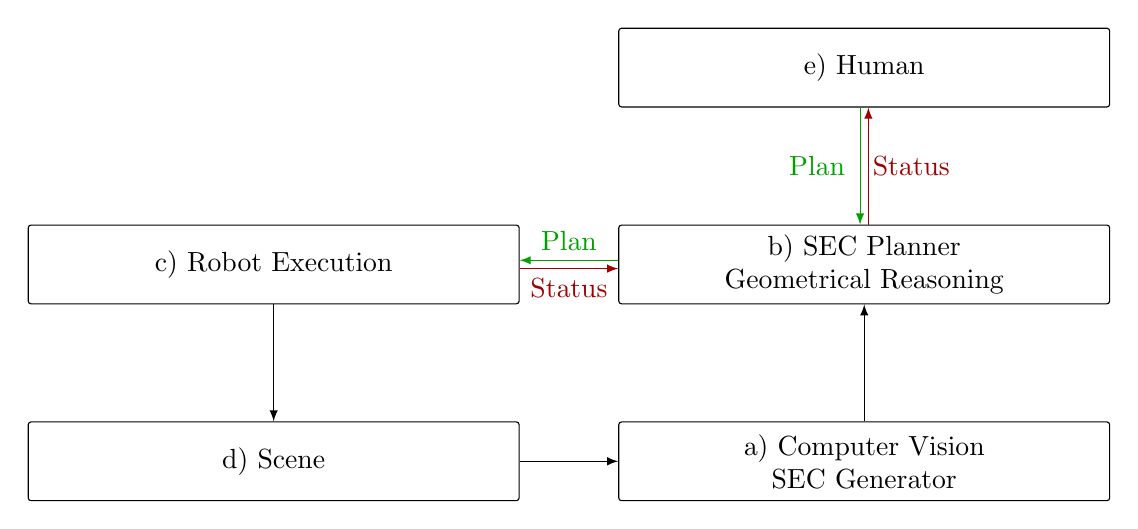
\begin{tikzpicture}[node distance=2.5cm, auto]
	\node [block] (scene) {d) Scene};
	\node [block, right of=scene, node distance=7.5cm] (computervision) {a) Computer Vision\\SEC Generator};
	\node [block, above of=computervision] (planner_sec) {b) SEC Planner\\Geometrical Reasoning};
	\node [block, above of=planner_sec] (planner_human) {e) Human};
	\node [block, above of=scene] (robot) {c) Robot Execution};

	\draw [arrow] (robot.south) to (scene.north);
	\draw [arrow] (scene.east) to (computervision.west);
	\draw [arrow] (computervision.north) to (planner_sec.south);

	% Planner SEC
	\draw [arrow, color=green1] ([yshift=0.15em] planner_sec.west) to node[arrowtext, above, name=plan] {Plan} ([yshift=0.15em] robot.east);
	\draw [arrow, color=red1] ([yshift=-0.15em] robot.east) to node[arrowtext, below, name=error] {Status} ([yshift=-0.15em] planner_sec.west);

	% Human
	\draw [arrow, color=red1] ([xshift=0.15em] planner_sec.north) to node[arrowtext, right, name=error, xshift=-0.8em] {Status} ([xshift=0.15em] planner_human.south);
	\draw [arrow, color=green1] ([xshift=-0.15em] planner_human.south) to node[arrowtext, left, name=plan, xshift=0.8em] {Plan} ([xshift=-0.15em] planner_sec.north);
\end{tikzpicture}

  \caption{Action perception loop of the presented system. First, d) the scene is recorded by a) a computer vision system: Here object segmentation, recognition, tracking, and eventually \gls{ac:sec} extraction takes place. The Semantic Event Chain, as well as a labeled Point Cloud, is given to the b) \gls{ac:sec} planner. The planner creates a plan based on a goal provided by e) a human being. The plan is given to c) a robot, which in turn will try to execute it. When encountering an error, \eg the touching relations have changed in an unexpected way, an error signal is returned. The plan is recomputed or, if no plan is found, the error signal is escalated to the human.}
  \label{fig:sec_usingaffordanceforplanning_plannerstructure}
\end{figure}


A schematic overview of the planning algorithm is shown in \figref{fig:sec_usingaffordanceforplanning_planneroverview}.
The semantic relations of the current scene, as analyzed by computer vision algorithms, are used as a) first input.
The second input b) is given to the planner in form of a target action, \eg \action{pick and place object A on top of object B}.
As the action has defined preconditions, the goal state can be derived from the current scene in form of a second \gls{ac:sem}.
The aim of the planner is now to find a set of ordered actions, which will transfer the current scene to the goal state using a Semantic Event Chain.


Both \glspl{ac:sem} are handed to the c) simulator.
Here, a tree is created.
At the very beginning of the planning stage, it has only one branch, the root, which is the input of the current scene.
In a trivial case the current scene already allows for the target action, which means all preconditions of the goal state are fulfilled by the current \gls{ac:sem}.
In this case ``Success'' is reported and a plan is handed to the robot - which consists of doing nothing except the requested action.
If not all preconditions are fulfilled, it is checked in d/lea) which actions are allowed given the current scene.
All allowed actions are appended to the tree as new leaves.
In e) it is analyzed whether these branches contain loops. 
If so, they are removed.
Also, branches that are too long are terminated.
The maximum length is given to the planner as a user-defined threshold.


\begin{figure}[]
  \centering
  % Define block styles
\tikzstyle{block} = [draw, rectangle, text centered, text width=6cm, minimum height=1cm, rounded corners=true]
\tikzstyle{blockSmall} = [draw, rectangle, text centered, text width=2cm, minimum height=1cm, rounded corners=true]
\tikzstyle{arrowtext} = [text width=4em, text centered]
\tikzstyle{arrow} = [draw, -latex]

\definecolor{red1}{RGB}{160,0,0}
\definecolor{green1}{RGB}{0,160,0}
\definecolor{blue1}{RGB}{0,0,160}
	      
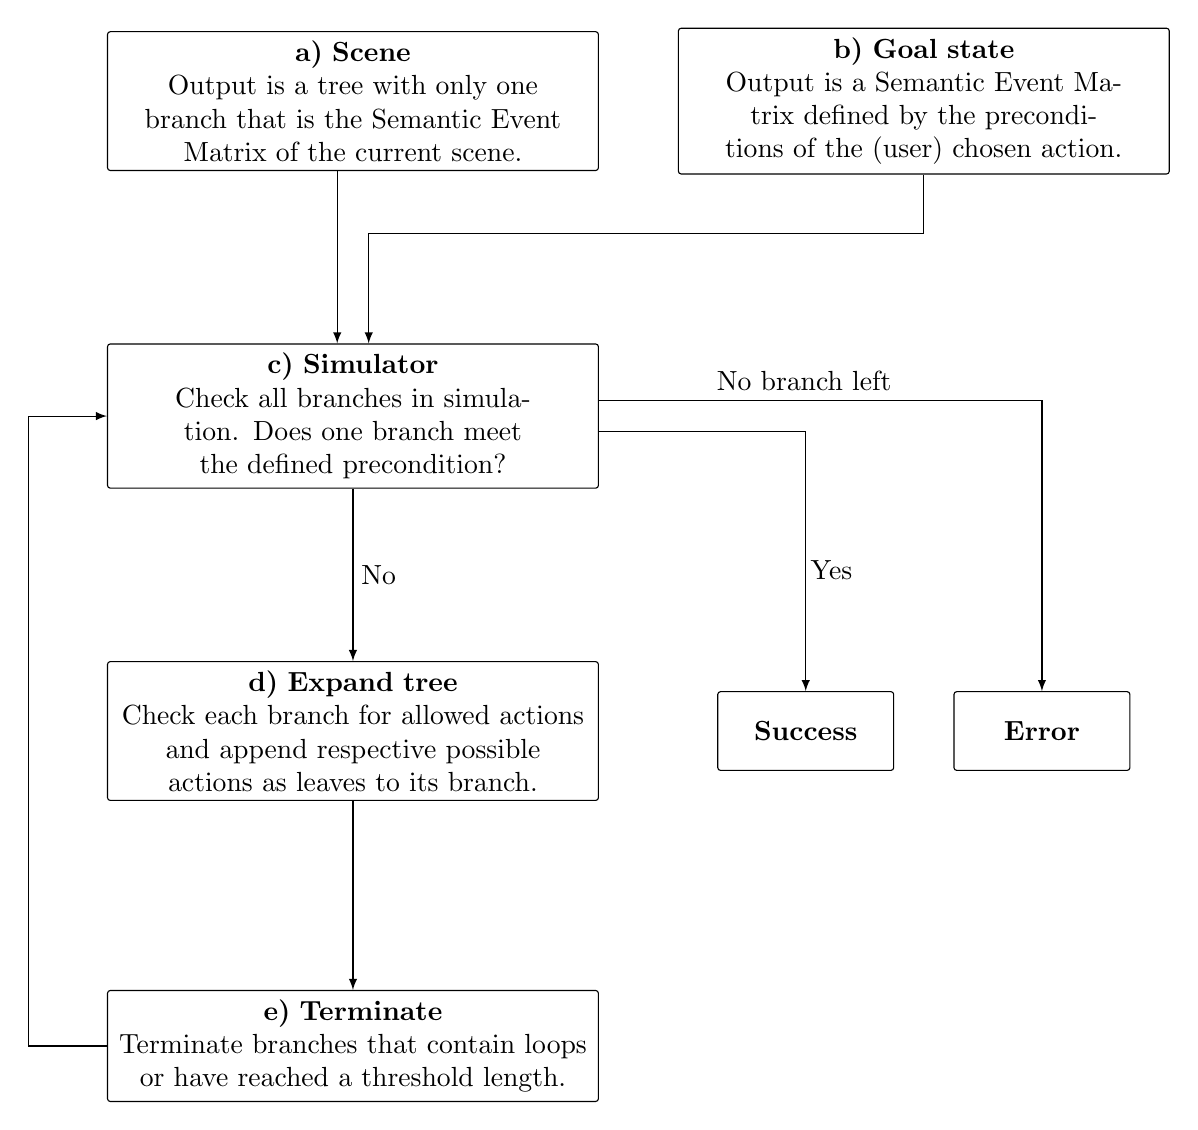
\begin{tikzpicture}[node distance=4.0cm, auto]
  \node [block] (scene) {\textbf{a) Scene}\\Output is a tree with only one branch that is the Semantic Event Matrix of the current scene.};
  \node [block, right of=scene, node distance=7.25cm] (goalstate) {\textbf{b) Goal state}\\Output is a Semantic Event Matrix defined by the preconditions of the (user) chosen action.};
  
  \node [block, below of=scene] (check) {\textbf{c) Simulator}\\Check all branches in simulation. Does one branch meet the defined precondition?};
  \node [block, below of=check] (tree) {\textbf{d) Expand tree}\\Check each branch for allowed actions and append respective possible actions as leaves to its branch.};
  \node [block, below of=tree] (terminate) {\textbf{e) Terminate}\\Terminate branches that contain loops or have reached a threshold length.};

  \node [blockSmall, below of=goalstate, xshift=-1.5cm, node distance=8cm] (success) {\textbf{Success}};
  \node [blockSmall, below of=goalstate, xshift= 1.5cm, node distance=8cm] (error) {\textbf{Error}};

  \draw [arrow] ([xshift=-0.2cm]scene.south) to ([xshift=-0.2cm]check.north);
  \draw [arrow] (goalstate.south) |- ++(0,-0.75cm) -| ([xshift=+0.2cm]check.north);

  \draw [arrow] ([yshift=-0.2cm]check.east) -| node[arrowtext, right, name=plan, xshift=-0.5cm, yshift=-1.75cm] {Yes} (success.north);
  \draw [arrow] ([yshift=+0.2cm]check.east) node[arrowtext, above, name=plan, xshift=2.2cm, yshift=-0cm] {No~branch~left} -| (error.north);

  \draw [arrow] (check.south) -- node[arrowtext, right, name=plan, xshift=-0.5cm] {No} (tree.north);
  \draw [arrow] (tree.south) -- (terminate.north);
  \draw [arrow] (terminate.west) |- ++(-1.0cm, 0) |- (check.west);

	%\draw [arrow, color=green1] ([xshift=-0.15em] planner_human.south) to node[arrowtext, left, name=plan, xshift=0.8em] {Plan} ([xshift=-0.15em] planner_sec.north);
\end{tikzpicture}

  \caption{In a) the scene is recorded and the current semantic relations are extracted. b) The goal state to the planner consists of the preconditions of the goal action that is to be performed. a) and b) are given to the c) simulator: Here, it is checked whether the preconditions of the goal state are met. If so, the plan may be executed on the robot. If no branch is left to check and no plan is found, an error message is sent. Else, the tree is expanded in d). Each branch is simulated using the postconditions from \tabref{tab:sec_usingaffordanceforplanning_postconditions}. Then, all possible actions are appended to the branch as leaves. Lastly, in e) branches that contain loops or are too long are terminated.}
  \label{fig:sec_usingaffordanceforplanning_planneroverview}
\end{figure}


The tree is then given again to the c) simulator.
The simulator begins at the root of the tree, which is the current scene.
It takes the first branch and simulates the outcome.
If the outcome fulfills all preconditions, this solution is presented to the user.
Otherwise, all afforded actions of the simulated state are again appended to the current branch as leaves in d).
This process is repeated for all branches.
If no branch is left to check, because all have reached the user-defined threshold length, an error is reported.


This means, if one action cannot be achieved immediately, afforded actions from the ontology are tried.
Iteratively, a tree is created until a solution is found or an exit criterion is met.
Naturally, the here created tree grows large very fast, especially in cluttered scenes with many possible combinations of objects and actions.
To minimize computational time, loop detection is implemented.
The algorithm refers to loops when the same \acrlong{ac:sem} appears in one \acrlong{ac:sec} more than once.
Second, structural changes need to be performed to change a relation matrix, \ie \action{drawing} on an object, will not make it possible to \action{pick and place} it later on.
As suggested in~\cite{navadaansaripatil2011, winandsbjornssonsaito2010} an additional flag ``changes structure of Semantic Event Chain'' is attached to each action.
Only if one of action contains this flag, it is added to the tree.
This, again, minimizes computational complexity.


Next, the solution that is found first is not necessarily the best one and there is the possibility that several branches lead to the requested goal state.
Reporting all solutions, which have a length below the user-defined threshold, calls for a measure for the best set of actions.
As in Semantic Event Chains only very little structural information is stored, it is very hard to determine even the approximate trajectory length a robot has to execute.
This makes it near to impossible to define a fitness function.
However, one can look at the total number of actions that need to be performed and at the total number of changing touching relations, \ie the total length of all Semantic Event Chains.
This measure comes close to the execution time and allows for ranking all solutions from ``least complex'' to ``worst'' solution.
